\section{Algebraic Multigrid Preconditioners\label{AMG}} 
%
%MultiGrid methods are widely used as preconditioners of iterative
%Krylov solver for sparse linear systems. 
%They are very efficient methods, having linear computational
%complexity and hence perfect scalability, when 
%sparse and large linear systems stemming
%from the discretization of some scalar elliptic Partial Differential
%Equations (PDEs) have to be solved~\cite{Vassilevski2008}. 
%Many efforts are related to extend their efficient applicability also
%to more general systems, in particular in the direction of a complete
%algebraic approach, where no information on a possible geometric
%origin of the problem is exploited. In this last case, they are called
%Algebraic MultiGrid (AMG) or Algebraic Multilevel
%methods~\cite{Stuben2001}. 
Multigrid methods achieve  their efficiency by the recursive application
of two complementary processes: \emph{relaxation} and \emph{coarse-grid
correction}.
%
\begin{figure}[t]
\begin{center}
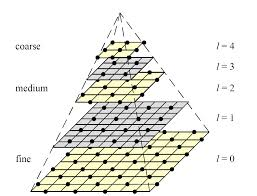
\includegraphics[width=.75\textwidth]{multilevel.png}
\caption{A MultiGrid hierarchy.\label{hierarchy}}
\end{center}
\end{figure}
%
Relaxation consists in the application of an iterative method, such as
Jacobi or Gauss-Seidel, to reduce highly oscillatory error components,
while the coarse-grid correction corresponds to the solution of the
resulting residual equation in an appropriately chosen coarse space,
aimed at reducing the leftover error components. The recursive application
of this procedure leads to a \emph{multilevel hierarchy} of spaces,
depicted in Fig.~\ref{hierarchy}. 

In the classical multigrid approach, the coarser grid and the interpolation
operator for transferring the coarse-grid solution to the original (fine) grid are
predefined by the geometry of the problem. Conversely,
AMG methods address the setup phase, known as~\emph{coarsening process},
in an automatic way, without using explicit knowledge of the
problem which the linear system originates from, and relying only on the entries of
the system matrix. Here we consider
an algebraic coarsening process based on the aggregation strategy,
where coarse-grid unknowns are aggregates of original
unknowns. In particular, the AMG preconditioners available in the MLD2P4
library~\cite{mld-toms} rely
on a decoupled version of \emph{the smoothed aggregation} algorithm
described in~\cite{BrezinaVanek96,BrezinaVanek99}. This procedure is
currently implemented on the host CPUs; for the sake of space,
we refer the reader to~\cite{mld2p4-2-guide} for details on the related
algorithm and its parallel implementation.

Our aim here is to identify the main linear algebra
operations needed for the application of the AMG preconditioner with
a Krylov solver, since the efficient implementation of these operations on
GPUs is the main focus of this work. 

The application phase of an AMG preconditioner is also known as
multigrid cycle. The most widely used one is the so called symmetric
V-cycle, described in Fig.~\ref{Vcycle}, where the AMG hierarchies of
$nlev$ prolongator operators $P^k$ and of corresponding coarse
matrices, obtained by the standard variational approach
$A^{k+1}=(P^{k+1})^TA^kP^{k+1}$, have been built in the setup phase.
%
\begin{figure}[t]
\begin{center}
\framebox{
\begin{minipage}{.85\textwidth}
\begin{tabbing}
\quad \=\quad \=\quad \=\quad \\[-3mm]
procedure V-cycle$\left(k,A^k,b^k,x^k\right)$ \\[2mm]
\>if $\left(k \ne nlev \right)$ then \\[1mm]
\>\> $x^k = x^k + (M^k)^{-1} \left(b^k - A^k x^k\right)$ \\[1mm]
\>\> $b^{k+1} = (P^{k+1})^T\left(b^k - A^k x^k\right)$ \\[1mm]
\>\> $x^{k+1} =$ V-cycle$\left(k+1,A^{k+1},b^{k+1},0\right)$ \\[1mm]
\>\> $x^k = x^k + P^{k+1} x^{k+1}$ \\[1mm]
\>\> $x^k = x^k + (M^k)^{-T} \left(b^k - A^k x^k\right)$ \\[1mm]
\>else \\[1mm]
\>\> $x^k = \left(A^k\right)^{-1} b^k$\\[1mm]
\>endif \\[1mm]
\>return $x^k$ \\[1mm]
end
\end{tabbing}
\end{minipage}
}
\caption{V-cycle preconditioner.\label{Vcycle}}
\end{center}
\end{figure}
%
$M^k$ represents the matrix
operator corresponding to the basic iterative method applied as smoother
at level $k$. 

The main computational kernels in the application of the preconditioner
are the sparse matrix-vector multiplication and the inversion of  $M^k$.
In the simple case of Jacobi method, $M^k=diag(A^k)$ and hence
inverting $M^k$ corresponds to a highly parallel vector
update operation. On the other hand, more robust iterative methods,
such as the Gauss-Seidel method or incomplete factorizations, are
often required to improve the convergence of the preconditioned solver
applied to general linear systems. In these cases, the inversion of
the corresponding matrix operators requires the solution of triangular
systems, which is a sequential kernel. Therefore, an
efficient parallel implementation of the V-cycle is
strictly related to the availability of iterative
methods which can be formulated in terms of sparse matrix-vector multiplication (SpMV)
and, possibly, vector updates, and to an efficient implementation of the sparse
matrix-vector multiplication.
